
\chapter{表面法线提取}

本章首先介绍我们为提取零件法线信息设计的硬件设备,该设备通过不同模块的组合,
能够精确地获取到算法所需不同方向光源下的零件照片。
随后我们将描述如何通过该设备得到的数据来计算物体法线,这一计算过程主要包括三部分,
分别是对相机成像的校正算法、对光线损失的补偿算法和最终零件表面法线的计算算法。
其中校正算法又包括白平衡校正、颜色校正和畸变校正。

\section{硬件设计与实现}
\label{section:yingjianshebeidesheji}

为了精确地计算表面法线,算法要求获取特定角度光源下的零件表面照片,为此本文设计了一款精密零件照片捕捉设备,该设备通过良好的物理设计和软件驱动,可以完成对算法所需数据的采集。整个设备的硬件结构如图\ref{zheguangmokuai}所示,主要包含遮光模块、平台模块、灯光模块、拍照模块和控制模块五个模块,每个模块的设计和功能介绍如下:
\begin{figure}[htbp]
\centering
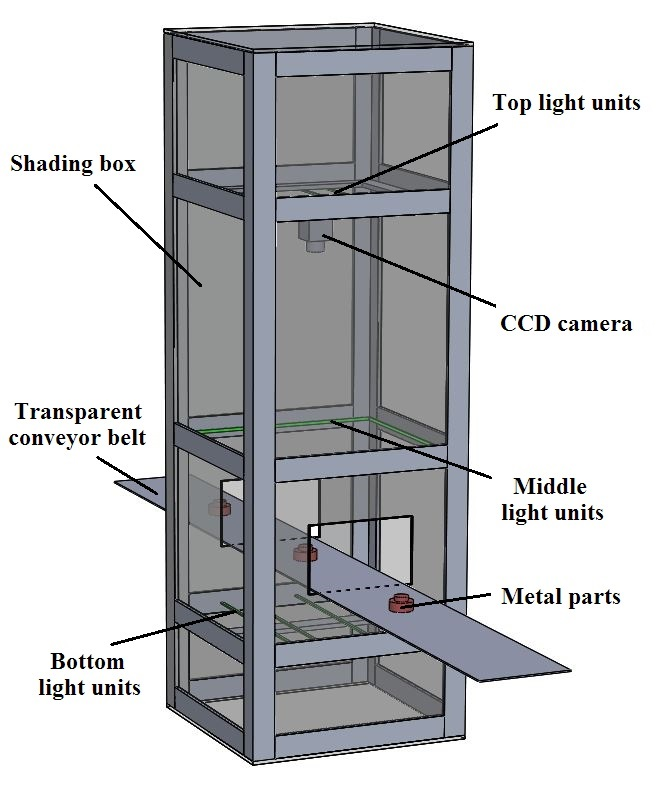
\includegraphics[width=0.6\textwidth]{figures/zheguangmokuai.png}
\caption{设备结构图}\label{zheguangmokuai}
\end{figure}
\begin{enumerate}
\item 遮光模块:为了捕捉特定入射角度光源下的照片,我们需要提供一个屏蔽其它光源的拍摄环境,
为此我们将整个设备设计在一个($60cm\times 60cm\times 110cm$)的遮光箱(如图\ref{zheguangmokuai}内标记Shading box部分)内。
为使设备稳固和耐用,遮光箱用金属材质搭建框架,并在框架上面覆盖了黑色塑料板,形成一个密闭的环境。
同时,为了避免遮光箱箱体材质对光的反射,影响灯光环境,我们使用一种黑绒布材料覆盖在遮光箱内部,该材料具有吸光的特性,能削弱遮光箱本身材质对光照环境的影响。
\item
平台模块:由一块固定在距遮光箱底部
$10cm$处的一个白色亚力克匀光板组成,用来放置需要扫描的零件,
在应用到零件生产流水线上时,可以用一个传送带(图\ref{zheguangmokuai}中Transparent conveyor belt)替代。
该匀光板放置物体的一面为磨砂面,反射效果较弱,可以削弱对入射光的反射,减小对光照环境的影响。
\item
灯光模块:该模块为拍摄提供特定的灯光环境,环境要求灯光为满足一定入射角度的平行光源,
同时尽可能的避免散射和衰减。此模块包括周围四组光源(图\ref{zheguangmokuai}中Middle light units)、顶部光源(图\ref{zheguangmokuai}中Top light units)以及覆盖在光源上的的CPL滤光膜。所有的光源均由一组LED灯带组成,既保证了光源质量,又节约了成本。
周围四组光源设置在平台模块上$20cm$处的遮光箱四壁,
通过一个金属槽卡住LED灯带,分别从放置物体平台的前(东)、后(西)、左(南)、右(北)
四个方向以${45}^{\circ}$角照射平台中央。拍摄时,当东部灯组亮起,零件照片呈现出上半部分较亮,下半部分较暗的特点,西部灯光组亮起则与之相反;南部灯组亮起,捕获的照片左半部分会较亮,右半部分较暗,北部灯组亮起来时呈相反特点。顶部灯组由四条LED灯带组成,固定在相机镜头下$3cm$处,垂直照向平台中心。CPL滤光膜具有选择性通过某个方向光线的功能,配合数码相机的偏光镜头能起到滤除高光的作用。我们在所有的灯带上均放置了滤光膜,搭配相机的偏光镜使用,滤除金属零件表面高光。
\item
拍照模块:拍照模块包括一款单反相机和偏光镜镜头。本文所用相机为Nikon D9000。相机固定于遮光箱顶部正中间位置,使镜头正对着平台正中心。在镜头下方放置一个偏光镜头,通过步进电机控制其位置,电机正向转动,可将偏光镜移到镜头下方,反向转动,可将偏光镜移开。
\item
控制模块:控制模块由单片机、继电器、步进电机和他们的配套驱动、电源组成。单片机分别于继电器和步进电机相连,用来控制继电器的开闭和步进电机的转、停、换向。继电器连在灯光线路上,被当做光源的开关,它的开闭代表着电路的通断,步进电机被用来控制偏光镜的位置。通过这种设计,
单片机输出不同的高低电平即可控制灯光的开闭和偏光镜的位置,而我们只需要将计算机连接到单片机上,通过控制单片机即可实现整个硬件设备的控制。
\end{enumerate}

完成所有模块的设计之后,通过这一设备即可对零件进行扫描,获取
拍照结果,其结果如图
\ref{caputure}
所示。
图\ref{caputure}中图组$(a)$
为使用了偏光镜和滤光膜滤除了高光之后的拍照结果,
图组$(b)$
为保留了高光得到的拍照结果。
图组$(a)$中
$North$表示北部灯光组亮起时的拍照结果,此时照片上半部分较亮,下半部分较暗,
记为$Image\_N1$;
$South$表示南部灯光组亮起时的拍照结果,此时照片下半部分较亮,上半部分较暗,
记为$Image\_S1$;
$West$表示西部灯光组亮起时的拍照结果,此时照片左半部分较亮,右半部分较暗,
记为$Image\_W1$;
$East$表示东部灯光组亮起时的拍照结果,此时照片右半部分较亮,左半部分较暗,
记为$Image\_E1$;
$Top$表示顶部灯光组亮起时的拍照结果,记为
$Image\_T1$。
保留高光时,
对应的图片分别记为$Image\_N2$、$Image\_S2$、$Image\_W2$、$Image\_E2$、$Image\_T2$。

\begin{figure}[htbp]
\centering
	\begin{minipage}[]{1.0\linewidth}
	\centerline{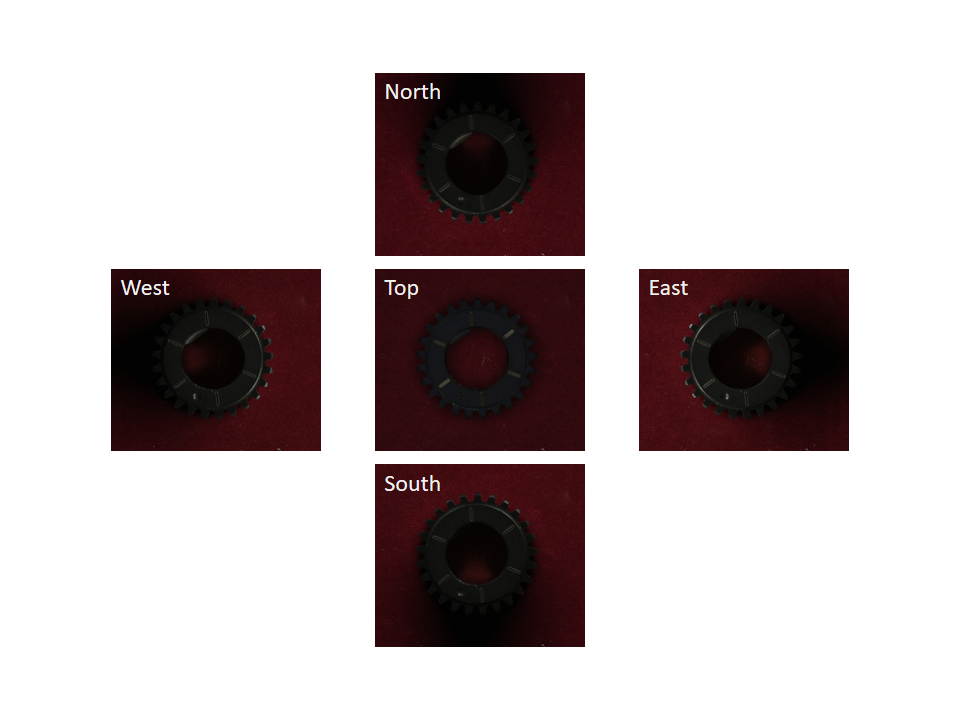
\includegraphics[width=1\linewidth]{figures/capturea.png}}
	\centerline{
		\footnotesize{(a)}}
	\label{caputurea}
	\end{minipage}
	\begin{minipage}[]{1.0\linewidth}
	\vspace{-1pt}
	\centerline{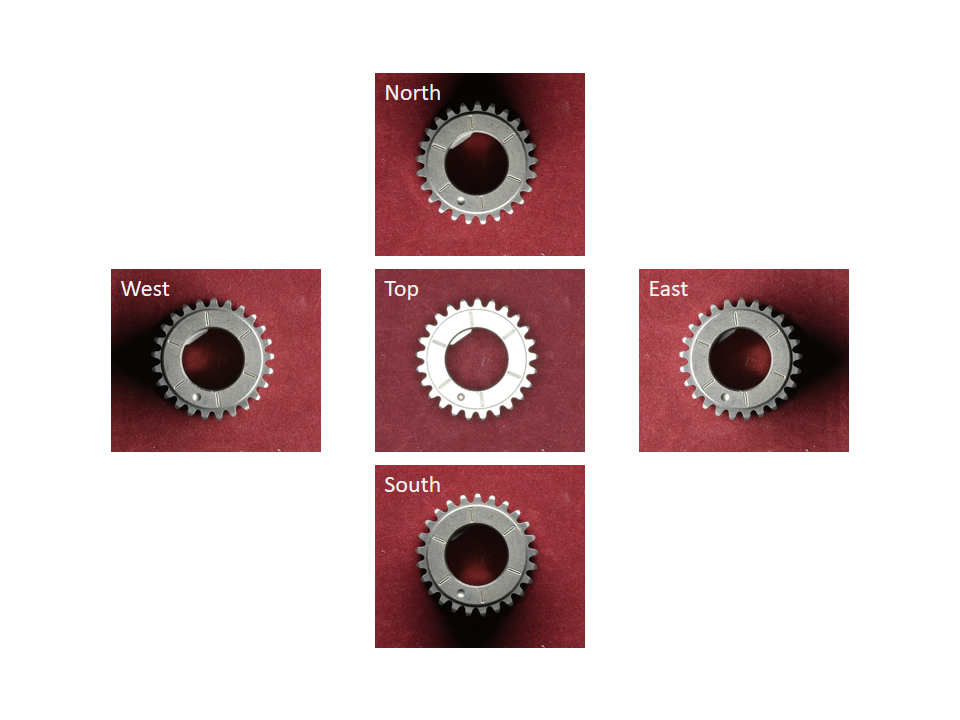
\includegraphics[width=1\linewidth]{figures/captureb.png}}
	\centerline{
		\footnotesize{(b)}
	}
	\label{caputureb}
	\end{minipage}
\caption{扫描结果:(a)表示滤除高光的结果,(b)表示保留高光的结果}
\label{caputure}
\vspace{-5pt}
\end{figure}

\section{算法设计与实现}

本节介绍提取零件表面法线的算法。该算法使用上节设备得到的零件照片作为输入,基于光线的反射原理计算零件表面
法线。同
时,为了优化照片的质量,提高零件法线的精度,本节首先对相机进行了
校正,这些校正包括白平衡校正、色彩校正、畸变校正;接着对方向光源
产生的损失进行了光线补偿,该补偿算法预存储了一套补偿数据,并利用
预存储的补偿数据对新的照片进行光线补偿;最后详细描述法线计算方法。
值得一提的是,我们的法线
提取算法不仅可以用来获取零件法线,也可以用来获取其他物体的法线。

\subsection{白平衡校正}

白平衡校正指在图像处理过程中,对原本为白色的物体进行色彩还原,使其在图片中也是白色,从而去除光源色温的影响。本文中白平衡校正用来去除LED灯带的色温。
白平衡校正有两个基础理论:灰度世界理论和完美反射理论。
白平衡算法大都基于这两个理论,
比如Xiaoqiang Li\cite{10.1007/978-3-642-37149-3_38}提出的算法就是对灰度世界算法的改进,
Lam 和Edmun Y\cite{lam2005combining}将这两个理论结合,提出了一种自动白平衡算法。

本文白平衡校正算法基于Weng\cite{weng2005novel}等人提出的校正算法,
并在此基础上作出优化。该算法分为两步,首先检测白点,接着用白点调整色温。
在校正前,我们首先计算图片$YC_b C_r$颜色空间的值,
计算公式如\eqref{eq:rgb2gray}所示,其中$R$、$G$、$B$分别代表原来$RGB$
色彩空间中三个通道的值,$Y$、$C_b$、$C_r$分别代表了$YC_b C_r$空间各个通道的值。
\begin{equation}\label{eq:rgb2gray}
\begin{split}
Y=(0.256\ast R)+ (0.504\ast G)+(0.098\ast B)+16\\
C_b=-(0.148\ast R)-(0.291\ast G)+(0.439\ast B)+128\\
C_r=(0.439\ast R)-(0.368\ast G)-(0.071\ast B)+128
\end{split}
\end{equation}
接着算法定义了一个$near-white$区域,并将该区域所有像素作为白点候选,
随后通过求解一系列约束条件得到最优白点集合。
论文中的算法需要统计所有$near-white$区域,
并进行一系列复杂的变换求解约束条件,大大限制了其速度,
并且约束条件以及$near-white$区域的选取都需要设定阈值,在不同情况下需要手动调整参数。
本文使用白卡辅助确定白点,
在确定白点过程中,
我们首先对照片中的白卡进行定位,识别出白卡所在位置,
接着选择白卡中白色区域作为白点候选,
从白点候选中确定最优白点集合。
在确定最优白点集合时,
我们只需要排除白点候选中的离群点即可得到最终结果。
这种优化有三点好处:一是无需手动设定参数;二是大大降低了白点统计的复杂度,提高了速度;三是白卡中的白色区域为已知真实白色,要比论文中定义的$near-white$区域更准确。
确定白点之后,算法使用Von Kries模型\cite{macadam1970sources}来调整图片。该模型首先计算通道增益,通道增益$R_{gain}$,$ G_{gain}$, $B_{gain}$可以根据公式\eqref{eq:gain}计算,
\begin{equation}\label{eq:gain}
\begin{split}
R_{gain}=Y_{max}/R_{avew}\\
G_{gain}=Y_{max}/G_{avew}\\
B_{gain}=Y_{max}/B_{avew}
\end{split}
\end{equation}
其中,$R_{avew}$、$G_{avew}$、$B_{avew}$分别代表白点集$Red$、$Green$、$Blue$三个通道像素值的均值,$Y_{max}$表示整张图片的最大亮度值。
接着使用公式\eqref{eq:brithnessadjust}对照片进行调整,
\begin{equation}\label{eq:brithnessadjust}
\begin{split}
R_{gain}=Y_{max}/R_{avew}\\
G_{gain}=Y_{max}/G_{avew}\\
B_{gain}=Y_{max}/B_{avew}
\end{split}
\end{equation}
公式中 $R$、$G$、$B$代表原图片中相应通道的像素值,$R^{'}$、$G^{'}$、$B^{'}$则代表了调整后图片对应通道的像素值。

\subsection{颜色校正}


颜色校正又称为色彩校正,是对图像的颜色进行调整,使其更接近真实色彩的过程。
人类在不同光照条件下对同一色彩感知到的结果相同,
被称为色恒定性,
然而成像系统不同于人类,并不具有这一特性,
它们所获图像的色受光源、物体反射率和成像系统的光谱响应函数影响,
因此相机在不同的光照条件下对同一物体拍摄得到的图像往往不同,
并且跟人眼观察结果也有差异。
为了避免成像系统的色彩偏差,必须对图像进行色彩校正。

颜色校正目前已有大量研究工作,Porikli\cite{weng2005novel}使用距离矩阵和模型函数的方法来对相机的颜色进行矫正,
Jinlong Lin\cite{porikli2003inter}等人提出了一种基于边缘检测的色偏校正算法,
利用彩色图像的边缘色度来进行颜色校正,
Hao Yu、Jian Wang\cite{yu2009color}等人则选择在Lab空间对颜色进行校正。

本文颜色校正基于设备提供的单一光照环境,因此算法不需要自适应其它环境,只需要针对我们的实验环境进行校正即可。
算法使用标准24色色卡辅助校正,
对于一块标准的24色色卡,
 每一块色卡中都包含24种色彩,分别位于24个矩形块中,拥有不同的$R$、$G$、$B$值,我们将第i种色彩的值记作$C_{org}^i$。
 标准色卡有固定的形状,
 可以使用边缘检测提取色卡照片中的直线,接着根据直线分割出不同的区域,得到色卡中不同区域的颜色值信息。
 对不同的区域i ,我们统计该区域的像素均值记为$C_{cap}^i$,显然,这里的$C_{org}^i$和$C_{cap}^i$都是三维向量,包含$R$、$G$、$B$通道的像素值信息。对应照片中色卡的像素值信息和其标准值,可以得到24个色彩值对,我们使用它们拟合一个函数$f(R,G,B)$,该函数的输入为照片的$R$、$G$、$B$通道值,输出为矫正后的像素值。


\subsection{畸变校正}

由于相机成像镜头固有的透镜效应,相机成像时会对真实的景象产生一种透视失真,被称为镜头畸变。随着镜头制造工艺的不断发展,人们通过不断改善镜头材质,优化光学设计,试图消除这种畸变,然而即使最先进的材质,最完善的设计,也难以完全消除畸变,必须借助镜头畸变校正算法进一步优化。

在计算机视觉领域,畸变校正算法已经发展的非常成熟,其中最成功的是张正友教授提出的张氏标定法\cite{zhang2000flexible},该方法现已被广泛应用于相机标定和畸变校正中。
Weng J,Cohen P\cite{weng1992camera}等人提出了先估计参数后迭代校正的两步校正方法,
Heikkila J 和Silven O\cite{heikkila1997four}等人则在Weng J等人算法的基础上进行扩展,
将两步扩展到四步,
使用额外的步骤补偿镜头的圆形特性引起的图像失真问题。
但是无论这些校正算法步骤如何,都需要估计相机参数。
相机参数分为内参、外参和畸变参数,
其中畸变参数是畸变校正中最重要的参数。
相机畸变参数包括径向畸变系数和切向畸变系数,
径向畸变是由于透镜本身的凹凸性质导致,光线在远离透镜中心的地方比靠近中心的地方更加弯曲;
切向畸变主要发生于成像仪被粘贴在摄像机上的时候,
这时成像透镜本身并不完全平行于成像平面。
畸变校正算法首先获取畸变系数,计算畸变系数对图像的作用矩阵,
通过对照片进行畸变作用相反的变换,得到消除畸变的矫正图像。

本文采用张氏标定法对相机标定,
算法只关注径向畸变。一般来讲,相机径向畸变较小,可以用主点(principle point)周围的泰勒级数展开的前几项进行描述,张氏标定法选择前两项来描述。
首先我们用待标定的相机拍摄多张包含棋盘格的照片,
拍摄时保证相机位置不变,每张棋盘格角度和位置各不相同,假设我们得到n张照片,接着
分别提取n张照片中棋盘格的$m$个角点,
根据相机成像原理可以得到$2mn$个等式,
对这$2mn$个等式使用最小二乘法求解,可以得到最优的径向畸变参数$k=[k_{1}$、$k_{2}]$,最后结合相机的内参和外参,进行极大似然估计得到更准确的畸变参数,将得到的参数保存起来,在需要的时候通过公式\eqref{eq:cortjibian}对照片进行畸变校正,
\begin{equation}\label{eq:cortjibian}
\begin{split}
p=p^{'}+(p^{'}-p_{0} )[k_{1} (x^{2}+y^{2} )+k_{2} (x^{2}+y^{2} )^{2} ]\\
q=q^{'}+(q^{'}-q_{0} )[k_{1} (x^{2}+y^{2} )+k_{2} (x^{2}+y^{2} )^{2} ]
\end{split}
\end{equation}
公式中,$(p,q)$代表畸变校正后的像素坐标,
$(p^{'}, q^{'})$
表示相机拍摄照片的像素坐标,
$k_{1}$、$k_{2}$表示张氏标定法中得到的相机畸变参数,
$(p_{0},q_{0})$
为主点的坐标。

\subsection{光线补偿}

虽然我们在设计硬件时充分考虑了光线的质量,
但是在拍摄时,仍然存在光线不均匀的情况,尤其是当需要拍摄的零件本身比较大时,光线损失会更加明显,严重影响法线的计算。因此我们需要对照片进行光线补偿,从而减少光线损失带来的误差。

已有的光照补偿算法如
\cite{贾灵芝2008基于自适应光线补偿的人脸检测算法,chen2006illumination,ruiz2008illumination,malassiotis2005robust,zheng2008intra,wiegand2003overview,tan2006intra,tan2007intra}中所提到的离散余弦变换、局部自适应模板匹配等从不同的角度对光照进行补偿,本文参考了这些方法,通过模板和函数方法进行光线补偿。

我们首先统计了不同颜色和不同灰度的材质在实验环境中所表现出来的光线损失情况,
结果如图\ref{fig:guangxiansunshi}所示,其中$(a)$、$(b)$、$(c)$、$(d)$分别代表了不同材质的光线损失图,从图中可以看出不同材质的光线损失程度不同,并且,往往材质亮度越低,光线损失越小,亮度越高,光线损失越大。

\begin{figure}[htbp]

\begin{minipage}{0.48\linewidth}
\centerline{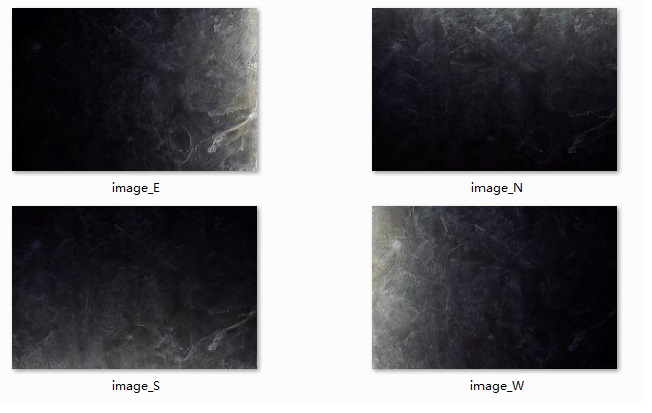
\includegraphics[width=1\linewidth]{figures/gaungxiansunshia.png}}
\centerline{(a)}
\end{minipage}
\begin{minipage}{0.48\linewidth}
\centerline{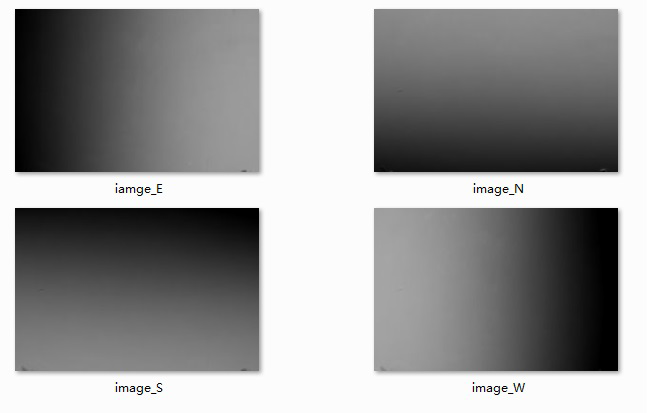
\includegraphics[width=1\linewidth]{figures/gaungxiansunshib.png}}
\centerline{(b)}
\end{minipage}


\begin{minipage}{0.48\linewidth}
\centerline{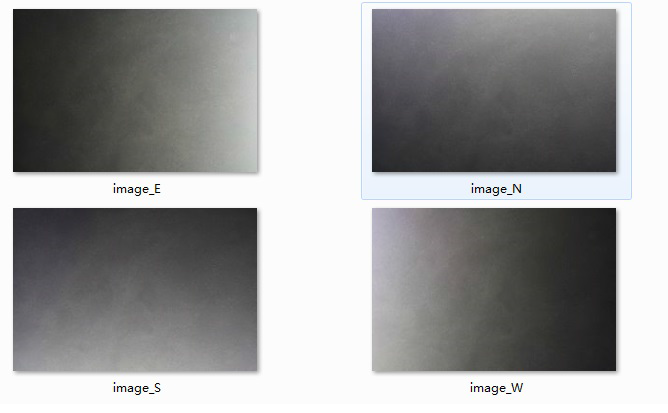
\includegraphics[width=1\linewidth]{figures/gaungxiansunshic.png}}
\centerline{(c)}
\end{minipage}
\begin{minipage}{0.48\linewidth}
\centerline{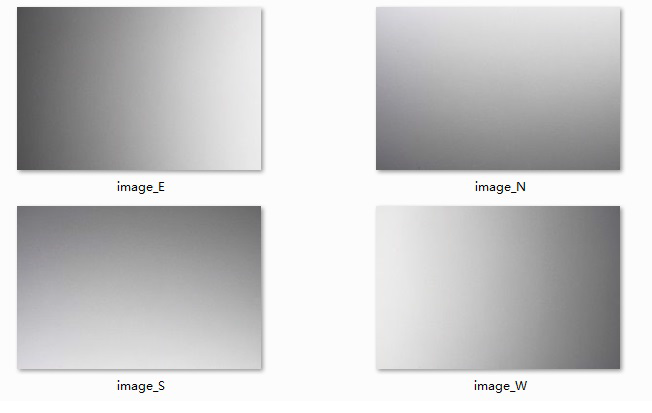
\includegraphics[width=1\linewidth]{figures/gaungxiansunshid.png}}
\centerline{(d)}
\end{minipage}

\caption{不同材质光线损失图}
\label{fig:guangxiansunshi}
\vspace{-3mm}
\end{figure}
{}
为了直观的展现光线损失和光源方向的关系,我们分别统计了照片在平行光源方向上的的衰减情况和垂直光源方向上的衰减情况,结果分别如图\ref{fig:guangxiansunshipingxing}和图\ref{fig:guangxiansunshichuizhi}所示,图中横轴表示统计方向上的位置,纵轴表示该位置上的亮度统计值,
图中不同颜色的曲线$(a)$、$(b)$、$(c)$、$(d)$分别代表了不同材质的损失曲线,
这些材质正是图\ref{fig:guangxiansunshi}中对应的材质,
$(E)$、$(W)$、$(N)$、$(S)$分别代表了东、西、北、南四个方向光源下的结果。
从图中可以明显看出,光线衰减在垂直光源方向上非常弱,但在平行光源方向上极为明显,并呈现出一种线性衰减的趋势。

\begin{figure}[htbp]

\begin{minipage}{0.48\linewidth}
\centerline{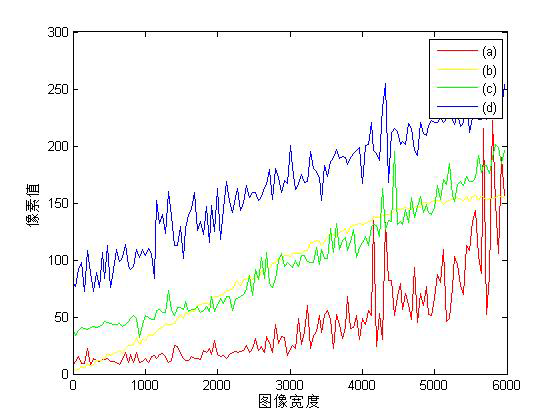
\includegraphics[width=1\linewidth]{figures/guangxianshuaijianduibituchuzhie.png}}
\centerline{(E)}
\end{minipage}
\begin{minipage}{0.48\linewidth}
\centerline{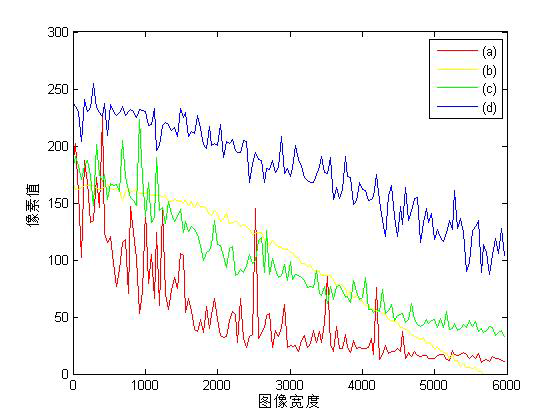
\includegraphics[width=1\linewidth]{figures/guangxianshuaijianduibituchuzhiw.png}}
\centerline{(W)}
\end{minipage}


\begin{minipage}{0.48\linewidth}
\centerline{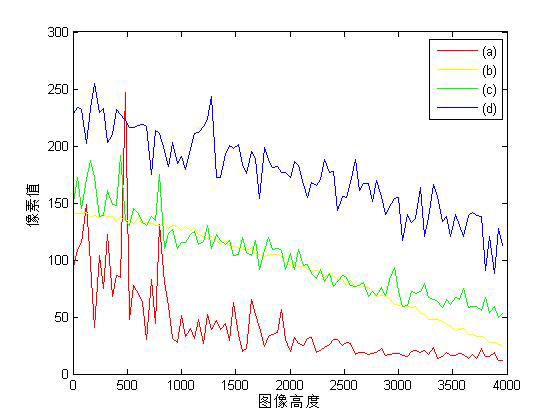
\includegraphics[width=1\linewidth]{figures/guangxianshuaijianduibituchuzhin.png}}
\centerline{(N)}
\end{minipage}
\begin{minipage}{0.48\linewidth}
\centerline{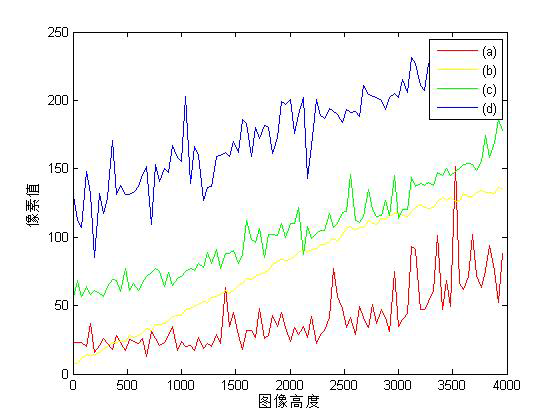
\includegraphics[width=1\linewidth]{figures/guangxianshuaijianduibituchuzhis.png}}
\centerline{(S)}
\end{minipage}

\caption{光线衰减统计图(平行光源方向)}
\label{fig:guangxiansunshipingxing}
\vspace{-3mm}
\end{figure}


\begin{figure}[htbp]

\begin{minipage}{0.48\linewidth}
\centerline{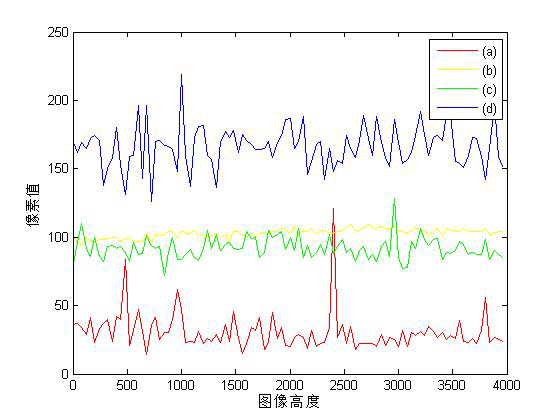
\includegraphics[width=1\linewidth]{figures/guangxianshuaijianduibitushuipinge.png}}
\centerline{(E)}
\end{minipage}
\begin{minipage}{0.48\linewidth}
\centerline{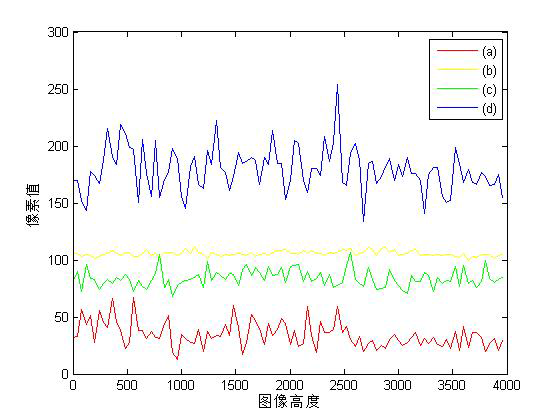
\includegraphics[width=1\linewidth]{figures/guangxianshuaijianduibitushuipingw.png}}
\centerline{(W)}
\end{minipage}


\begin{minipage}{0.48\linewidth}
\centerline{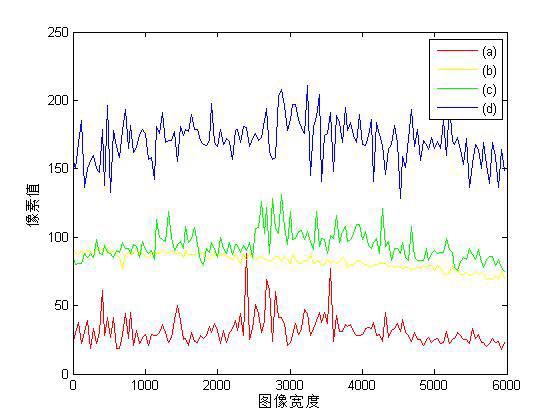
\includegraphics[width=1\linewidth]{figures/guangxianshuaijianduibitushuipings.png}}
\centerline{(N)}
\end{minipage}
\begin{minipage}{0.48\linewidth}
\centerline{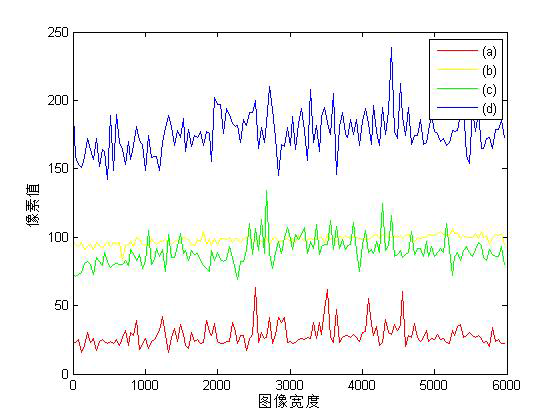
\includegraphics[width=1\linewidth]{figures/guangxianshuaijianduibitushuipingn.png}}
\centerline{(S)}
\end{minipage}

\caption{光线衰减统计图(垂直光源方向)}
\label{fig:guangxiansunshichuizhi}
\vspace{-3mm}
\end{figure}

在我们的实验环境中,相机和光源均固定不变,因此,我们可以在扫描材质前先计算一组光照补偿模板,然后针对不同的材质作出适当调整进行光线补偿。
因为我们只需对光线信息进行调整,并不涉及照片的色彩信息,
所以我们直接在亮度上进行计算,并且模板中也只保留亮度信息。
图像的亮度有多种表示方法,为了和其它步骤统一,我们使用$YC_b C_r$空间中的
$Y$分量代表亮度。

我们首先拍摄一组用来计算补偿模板的照片,这时相机直接拍摄匀光板,匀光板具有良好的光源分散性质,不容易造成光线损失。拍摄时,我们首先拍摄顶部光源下的照片,并将其作为没有损失的照片,记为
$Base$,
之后依次拍摄东部灯光组、西部灯光组、南部灯光组和北部灯光组下的待校正照片,
分别标记为${Adjust}_E$、${Adjust}_W$、${Adjust}_S$、${Adjust}_N$,
为了方便计算和节省存储空间,我们只保留他们的亮度值,
分别记为${Base}^L$、${Adjust}_E^L$、${Adjust}_W^L$、${Adjust}_S^L$、${Adjust}_N^L$。
接着我们使用${Base}^L$减去各个方向上的亮度值,得到不同方向光源上相对于Base的光线衰减信息,
为了保证补偿信息的非负性,我们为整体亮度增加一个偏差$\alpha$,
偏差的的小为${Base}^L$与${Adjust}_E^L$、${Adjust}_W^L$、${Adjust}_S^L$、${Adjust}_N^L$对应差值最小的$0.1\%$的均值。
如果结果仍为负0,我们直接将其置为0,认为此处没有损失,
最终补偿计算方法如公式\eqref{eq:guangxianbuchang}所示,
\begin{equation}\label{eq:guangxianbuchang}
{Comp}_d=\max ({0,{Base}^L-{Adjust}_d^L+\alpha }),\quad d\in \{E,W,S,N \}
\end{equation}
其中${Comp}_d$表示对应方向光源下的补偿信息,$\alpha$表示偏差,计算方法如公式\eqref{eq:paincahzhijisuan}所示,
其中$NMIN$表示集合对应差值的最小的$N_{min}$个值的集合,$N_{min}=N\times 0.001$,N表示图片的像素值总数。
\begin{equation}\label{eq:paincahzhijisuan}
\alpha =\frac {1}{N_{min}} \sum_{i}^{N_{min}}{Y_i},\quad Y_i\in NMIN
\end{equation}

考虑到不同亮度材质的光线损失程度不同,我们在校正时会对模板信息做相应调整。
根据前面的统计规律,我们使用线性函数对模板进行调整。当需要进行光线补偿时,记不同方向光源下的照片为
${Image}_d$,其中$d \in \{E,W,S,N\}$,
在顶部光源下拍摄的照片为${Image}_T$,我们用公式\eqref{eq:guangxianbuchangsuanfa}计算对应的补偿,
\begin{equation}
\label{eq:guangxianbuchangsuanfa}
{CImage}_d^L={Image}_d^L+\lambda*{Comp}_d*(avg({Image}_T^L)/avg({Base}^L))
\end{equation}
其中avg表示求平均值函数,${Image}_d^L$表示不同方向光源下照片的亮度值,
${CImage}_d^L$表示光线补偿后照片的亮度值,
$\lambda$为补偿强度参数,表示光线补偿的强度,
本文实验$\lambda$取$0.8$,如果需要增大补偿强度,可以将其调高。

\subsection{法线计算}


 Ryan Clark\cite{zarria.net}提出了一种在没有光线损失情况下的计算方法,
 他使用photoshop工具模拟了算法,并没有将该算法系统化,算法所得到的法线信息在细节和整体上都存在极大问题。
 并且,算法没有考虑光线损失对结果的影响。
 本文受该算法启发,利用光照反射原理计算法线,不仅此基础上增加了对光线损失的补偿,而且利用不同方向光源下的照片来计算,取得了更好地结果。

\begin{figure}[htbp]
\centering
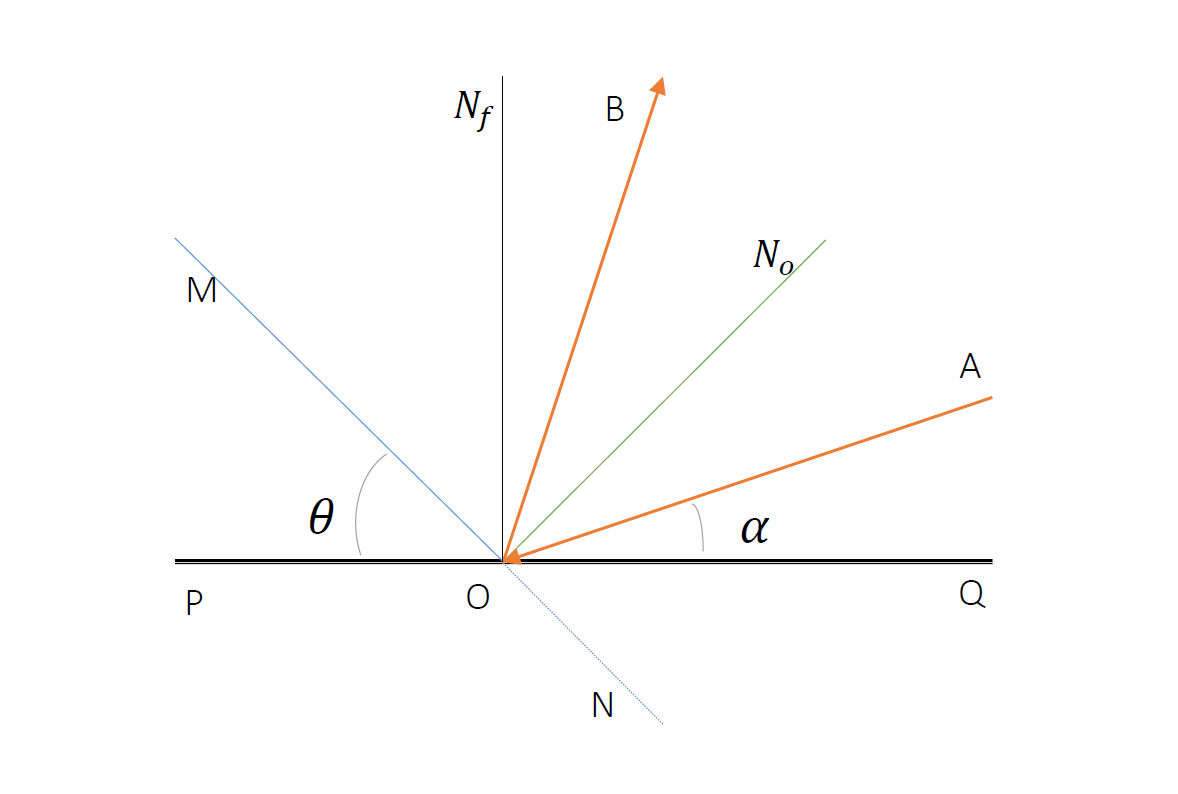
\includegraphics[width=0.8\linewidth]{figures/guangxianfanshetu.png}
\caption{光线反射原理图}
\label{fig:guangxianfanshetu}
\end{figure}

光照反射原理如图\ref{fig:guangxianfanshetu}所示,其中$PQ$表示水平面,
$MN$表示物体表面,
实线部分$MO$
为真实表面,
$ON$
是表面的延长,是为了方便观察和理解,
$\overrightarrow{AO}$为入射光,
$\overrightarrow{OB}$表示反射光,
$ON_f$
表示水平面的法线,垂直于
$PQ$,
$ON_o$表示物体表面法线,
垂直于$MN$,
$\angle POM$
为物体表面和水平面的夹角,记为
$\theta $,
$\angle AOQ$为入射光与水平面的夹角,记为
$\alpha$。在本系统中,实验环境固定,
相机镜头平行于水平面$PQ$,
不同方向光源和水平面的夹角为
$45^{\circ}$,
因此$\alpha=45^{\circ}$。
假设入射光线的强度为$I$,由
$\angle POM=\theta$和
$\angle AOQ=\alpha$易得
$\angle {BON}_f=2\theta+\alpha-90$
。根据光的反射原理,在不考虑其他介质对光的散射时,
反射到相机中的光线强度可以用公式\eqref{eq:guangxianqiangdu}来计算,
\begin{equation}
\label{eq:guangxianqiangdu}
I_{ref}=\lambda I* \cos (2\theta +\alpha-90)
\end{equation}
其中,$\lambda$表示光线反射率,
当光源相同时,光线反射率不变,
$\alpha$已知,为
$45^{\circ}$,
根据公式\eqref{eq:guangxianqiangdu},理论上反射到相机中的光照强度只有材质表面的倾斜角度有关,
光照强度反应在拍摄图片的亮度信息中,
因此拍摄照片的亮度信息必然只与材质本身的倾斜角度有关,
即亮度信息只和材质的法线有关,
根据这一推论,
我们可以使用四个不同方向光源下的照片来计算物体的法线。

我们首先获取不同方向光源下的照片
$Image\_E1$、$Image\_W1$、$Image\_N1$、$Image\_S1$,
使用光线补偿算法对其进行光线补偿,并得到其亮度信息,
记为
${Image}_E^L$、${Image}_W^L$、${Image}_N^L$、${Image}_S^L$,
接着我们创建两个新的三通道图
$NorthWest$和$SouthEast$
用来保存数据,其中
$NorthWest$的$R$通道保存
${Image}_W^L$,
$G$通道保存
${Image}_S^L$,
$SouthEast$的$R$通道保存
${Image}_E^L$,
$G$通道保存
${Image}_S^L$,
接着我们将$NorthEast$的色阶调整到$[0.0-0.5]$,
将SouthEast的色阶调整到$[0.5-1.0]$,
调整色阶的计算方法如公式\eqref{eq:tiaozhengsejie}所示,
其中$p$表示图像的像素值,
$a$为调整后色阶的上界,$b$为调整后色阶的下界,${p}^{'}$为调整后的像素值。
\begin{equation}
\label{eq:tiaozhengsejie}
{p}^{'}=p* (a-b)+b
\end{equation}
最后我们将$NorthWest$
和$SouthEast$叠加成一张法线图$Normal\_Temp1$,
叠加时使用公式
\eqref{eq:hunhetuxiang}
计算。
\begin{equation}
\label{eq:hunhetuxiang}
Normal\_Temp1=2* NorthWest* SouthEast
\end{equation}
这一法线图中包含了$R$和$G$通道的信息,由法线的归一化性质,我们可以根据R和G通道的值来计算B通道的值,计算方法如公式\eqref{eq:btongdaojisuan}所示,
其中$r$表示R通道像素值,$g$表示$G$通道的像素值,$b$表示$B$通道的像素值。
\begin{equation}
\label{eq:btongdaojisuan}
b=2.0* \sqrt{1.0-{(r-0.5)}^2+{(g-0.5)}^2}-1.0
\end{equation}

我们将$Image\_N2$、$Image\_S2$、$Image\_W2$、$Image\_N2$也使用上述处理方式,
可以得到有高光情况下的法线图$Normal\_Temp2$。
$Normal\_Temp1$滤除了高光,光线信息较弱,
细节部分表现较弱,但是整体结果较好,
$Normal\_Temp2$保留了高光信息,光线信息较强,细节表现明显,但部分区域容易出现法线的跳跃现象,因此我们使用alpha融合算法融合这两张法线图,得到最终法线,融合方法如公式
\eqref{eq:faxianronghe}所示。
\begin{equation}
\label{eq:faxianronghe}
Normal=(Normal\_Temp1+Normal\_Temp2)* 0.5
\end{equation}

实验结果如图\ref{fig:faxianjieguotu}所示,
其中$(a)$表示零件原图,$(b)$表示算法得到法线图,
我们的法线图既保留了细节信息又不会出现法线跳跃现象,具有良好的性质。

\begin{figure}[htbp]
\centering
\begin{minipage}{0.48\linewidth}
\centerline{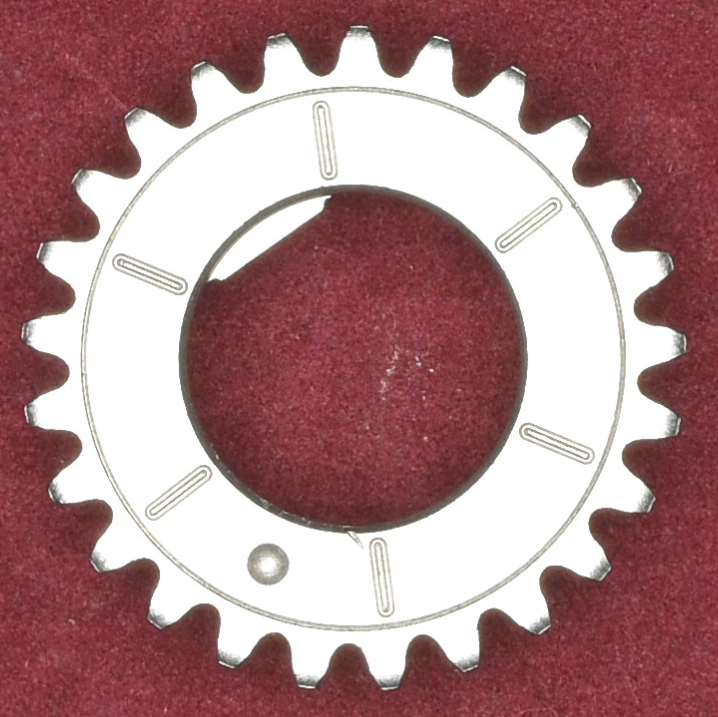
\includegraphics[width=1.0\linewidth]{figures/faxiantuyuantu.png}}
\centerline{(a)}
\end{minipage}
\begin{minipage}{0.48\linewidth}
\centerline{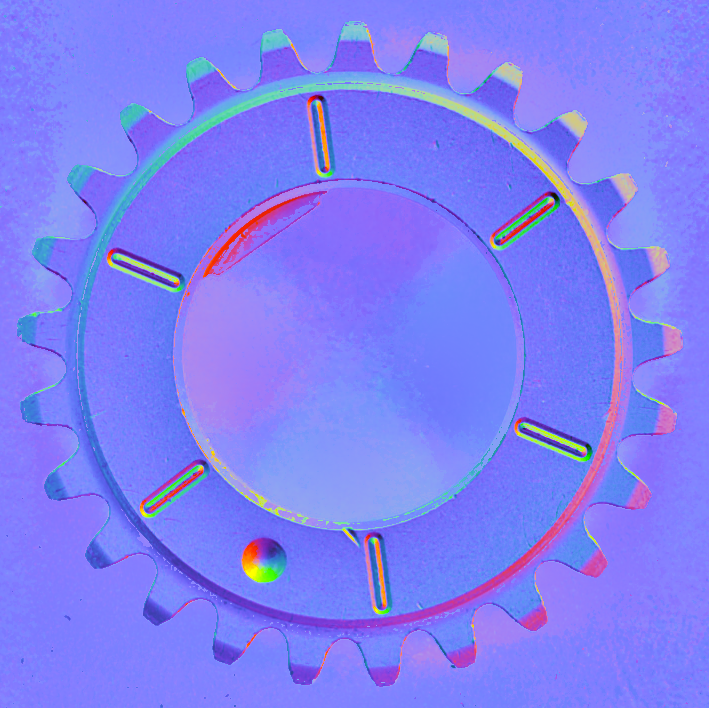
\includegraphics[width=1.0\linewidth]{figures/faxiantujieguo.png}}
\centerline{(b)}
\end{minipage}
\caption{法线提取结果图}
\label{fig:faxianjieguotu}
\end{figure}

\section{实验结果和分析}

本节首先介绍我们的硬件设备成品,接着介绍法线提取结果并与其他相关工作对比。
由于本章设计的法线提取算法不仅可以用于提取零件表面法线,还可以被扩展到任意材质的法线提取中,因此我们将它独立成一个模块,用于提取材质法线图,本节不仅包含零件表面法线提取结果,还包含了对其它材质的法线提取结果。

\subsection{硬件设备结果}

遵循\ref{section:yingjianshebeidesheji}节中的硬件设计,
我们给出了实现,并将其应用到了实际生产中。
设备由5个模块组成,这些模块被封装到一个白色的铝合金外壳中,如图\ref{fig:yingjianjieguo}所示,
$(a)$展示了设备的整体外观,
为了移动方便我们在设备底部安装了四个滚轮,
设备顶部可以打开,
如
图\ref{fig:yingjianjieguo}中$(b)$所示,打开之后可以看到固定在顶部的相机、滤光镜和顶部灯光组,
图\ref{fig:yingjianjieguo}中$(c)$展示了更清楚的结果,
设备中间部分如
图\ref{fig:yingjianjieguo}中$(a)$所示,
保留了一个门,门内
如$(d)$和$(e)$
所示,可以看到摆放材质的平台和不同方向的灯光组,
需要扫描的材质放在这个平台中间,灯光组以
${45}^{\circ}$
照向平台中间,从
图\ref{fig:yingjianjieguo}中$(b)$、$(c)$、$(d)$、$(e)$中都可以看到内部的黑色绒布,
这些绒布有吸光性质,可以减少了对光照的影响。

\begin{figure}[htbp]
\centering
\centerline{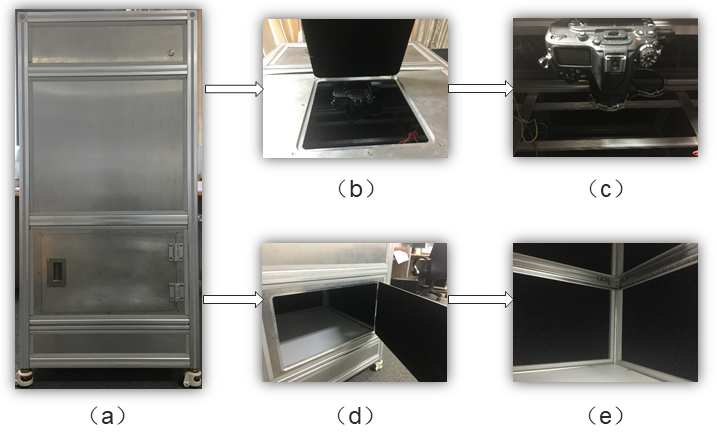
\includegraphics[width=1.0\linewidth]{figures/yingjianjieguo.png}}
\caption{硬件示意图}
\label{fig:yingjianjieguo}
\end{figure}

\subsection{法线提取结果}

在计算法线之前,我们先对相机进行白平衡校正、颜色校正、畸变校正以及光线补偿,保存它们的参数,用来对之后拍摄的照片校正。随着时间的推移,不论是相机还是光源都会有细微的变化,
为了保证参数的准确性,
在实际应用中我们定期的对相机进行这些校正,
更新校正参数。经验表明,至少三个月需要对设备重新校正一次。

获得校正参数之后,我们首先使用设备拍摄不同光源下的零件照片,
接着运行校正算法,最后计算零件表面法线。
为了拍摄不同光源下的零件照片,我们首先将目标放置在设备的平台中央,
接着使用程序控制硬件设备获取所需照片。
获取的过程分为两步,
第一步相机使用滤光镜,
程序分别控制亮起顶部灯光组、东部灯光组、西部灯光组、北部灯光组、南部灯光组并拍摄照片,并对照片进行校正,
保存结果为$Image\_T1$、$Image\_E1$、$Image\_W1$、$Image\_N1$、$Image\_S1$;
第二步中程序控制电机转动移开滤光镜,重复第一步中的步骤,对零件拍照和校正,
并存储结果为$Image\_T2$、$Image\_E2$、$Image\_W2$、$Image\_N2$、$Image\_S2$。
最后,使用这些数据运行法线提取算法,即可得到零件法线,
法线图结果如图\ref{fig:faxianjieguotu}所示。

在材质表面信息获取领域中,Vizoo3D xTex开始最早, 
并仍保持着业界领先水平,我们将本文结果与其结果作对比。
\begin{figure}[htbp]
\begin{minipage}{0.48\linewidth}
\centerline{
\includegraphics[width=1.0\linewidth]{figures/faxianduibia.png}}
\centerline{(a) Vizoo3D xTex的结果图 }
\end{minipage}
\begin{minipage}{0.48\linewidth}
\centerline{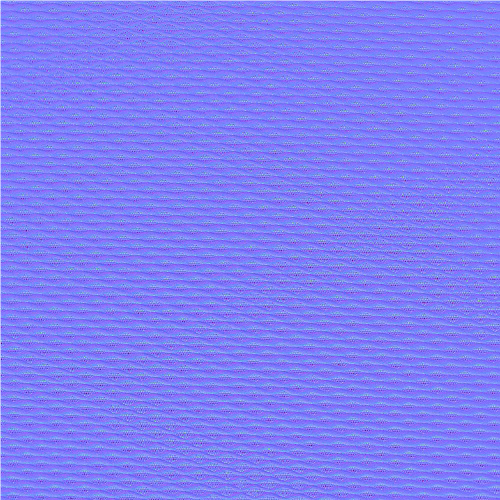
\includegraphics[width=1.0\linewidth]{figures/faxianduibib.png}}
\centerline{(b) 本文结果图}
\end{minipage}
\caption{法线结果对比图}
\label{fig:faxianjieguoduibi}
\end{figure}
我们首先得到他们对某一材质的法线提取结果,
然后使用我们拥有的最相似的材质提取法线并对比,结果如图\ref{fig:faxianjieguoduibi}
所示,其中
$(a)$表示Vizoo3D xTex得到的法线结果,
$(b)$为我们提取的法线结果,从图中可以看出这组法线都比较平整,
不存在褶皱等问题,
但是
$(a)$中的法线信息在中心处要比边缘部分模糊,
我们推测这可能是由于光线不均或光线损失导致,
而我们在法线计算过程中考虑了这一问题,因此我们的结果可以在不同区域保持一致。
图\ref{fig:faxianjieguotu}中展示了我们提取的其他材质的法线图,
其中$(a)$、$(b)$、$(c)$、$(d)$分别代表了不同材质的法线图,
从图中可以看出,对于不同的材质我们都能够得到较好的法线提取结果。
\begin{figure}[htbp]
\begin{minipage}{0.48\linewidth}
\centerline{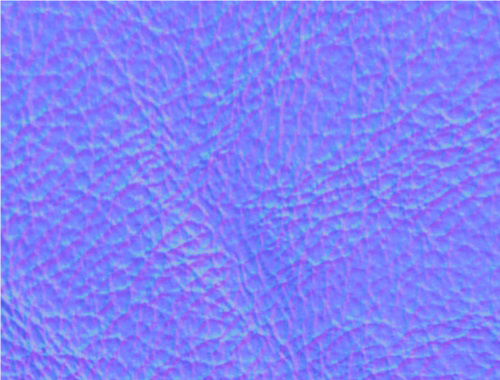
\includegraphics[width=1.0\linewidth]{figures/faxianjieguotua.png}}
\centerline{(a)}
\end{minipage}
\begin{minipage}{0.48\linewidth}
\centerline{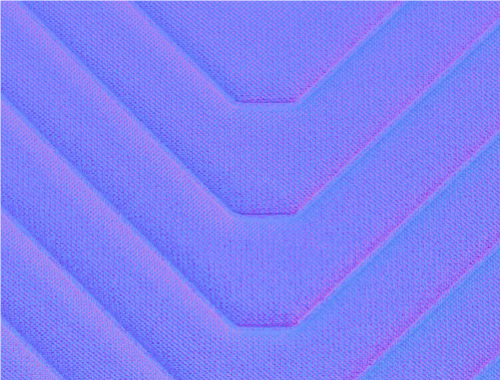
\includegraphics[width=1.0\linewidth]{figures/faxianjieguotub.png}}
\centerline{(b)}
\end{minipage}

\begin{minipage}{0.48\linewidth}
\centerline{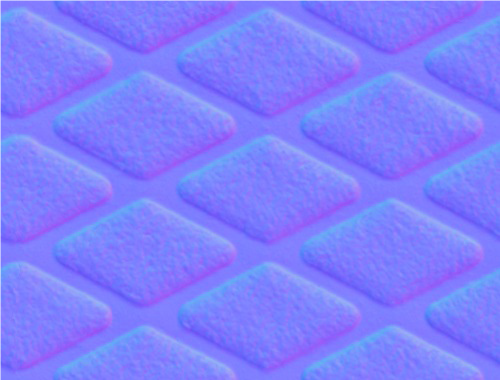
\includegraphics[width=1.0\linewidth]{figures/faxianjieguotuc.png}}
\centerline{(c)}
\end{minipage}
\begin{minipage}{0.48\linewidth}
\centerline{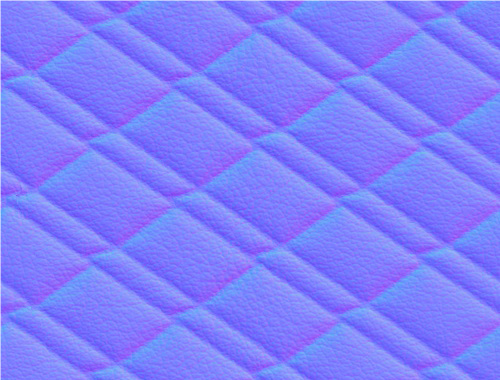
\includegraphics[width=1.0\linewidth]{figures/faxianjieguotud.png}}
\centerline{(d)}
\end{minipage}

\caption{法线结果图}
\label{fig:faxianjieguotu2}
\end{figure}